\documentclass[a4paper]{article}

\usepackage{siunitx}
\usepackage{graphicx}
\usepackage{hyperref}

\begin{document}
\title{Osborne 1 floppy drive emulator}
\date{July 2024}
\author{Archie Halliwell \and Lennart Leufgens \and Jun Muta \\
John Monash Science School}
\maketitle

\section{Abstract}

The Osborne 1 is a suitcase-sized portable computer released in 1981
is an important part in commputing history, being one of the first
widely available home computers. This project aims to allow the
sharing of programs for it over the internet. It sits in front of the
floppy disc module within the osborne with a small device that
interfaces with the motherboard and inserts data from a usb. This
replaces hard to find and costly 5.25'' floppy disks, which need to be
copied using legacy hardware, with usb drives, able to be loaded with
readily available files from the internet. The entire project's source
and documentation has been made readily available on github
(\url{https://github.com/archiecarrot123/osborne-floppy-emulator}) for
anyone who desires to recreate this project.

Our project came about from us trying to locate a copy of the CP/M
operating system on floppy disk for our school's Osborne, for which we
did not have any software available. Upon further research we realised
locating and creating these disks prohibitively difficult for
hobbyists. We chose to create a device that can emulate a floppy disk
from a usb instead of working with floppy disks directly because of
the technical limitations of floppy drives and their mechanical
complexity. 

\subsection{Problems}

The first problem we ran into was that a capacitor in the Osborne 1
exploded when it was first plugged in---the capacitor had absorbed
moisture over the years and this caused it to heat up and
explode---but this was easily fixed by replacing the capacitor with a
modern one.

The first board we had made turned out to be too big, and collided with
the power connector on the Osborne's logic board, so we had to design a second
version, for which we used more SMD components, enabling us to shrink
it to less than half the size.

\begin{figure}
  \centering
  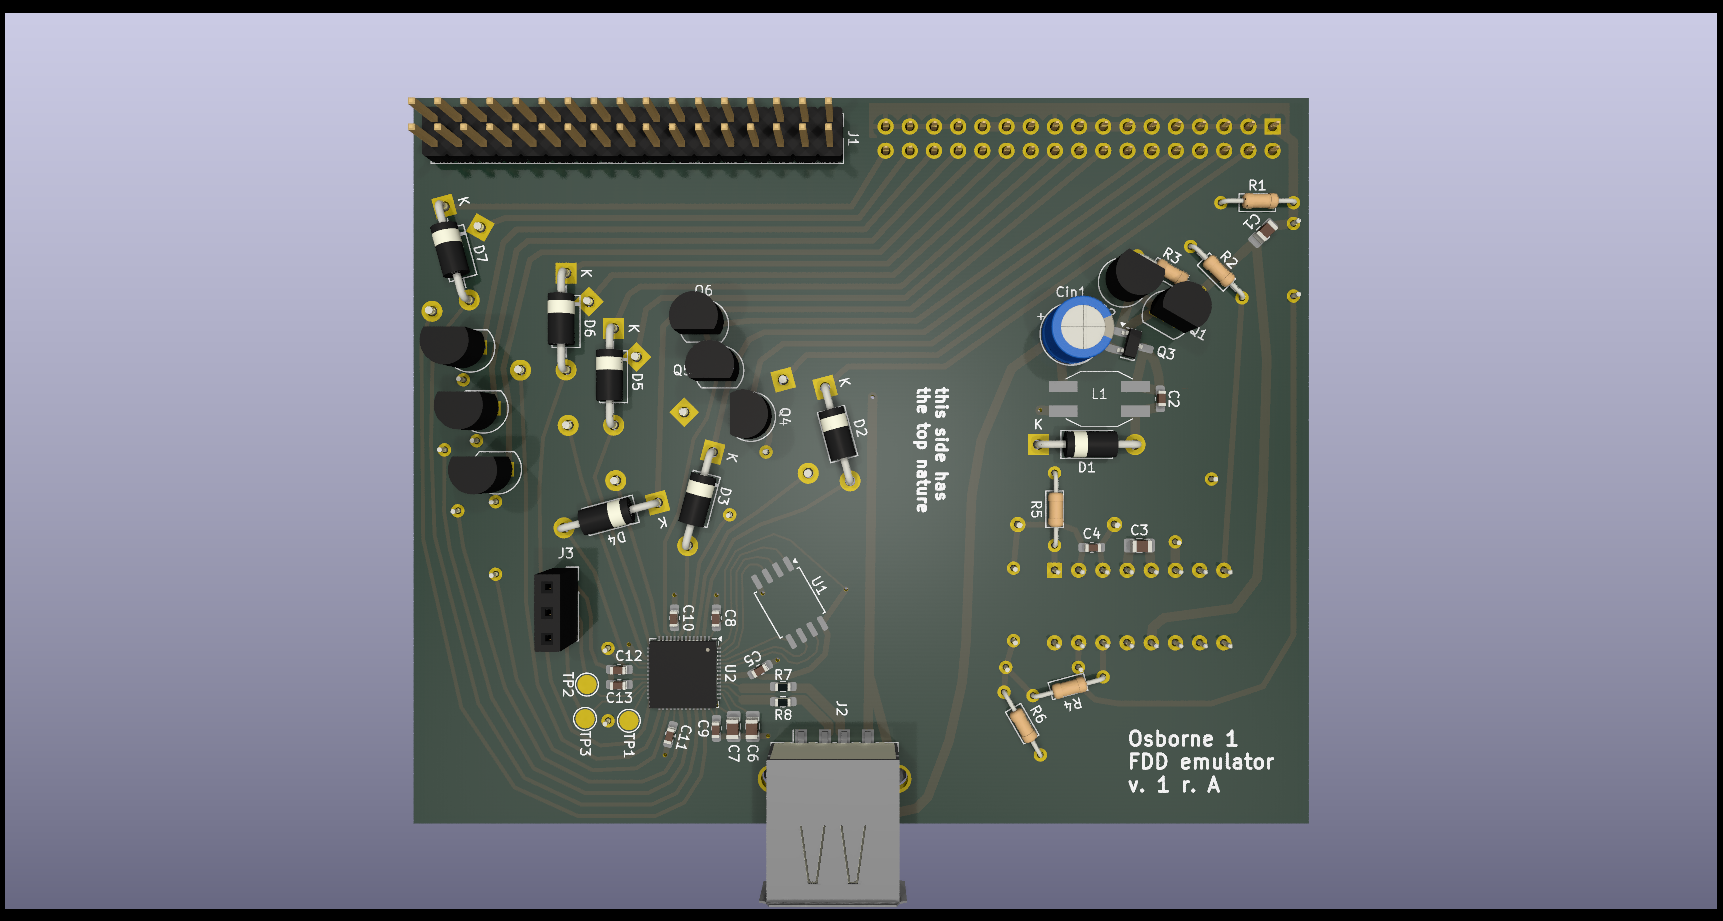
\includegraphics[height=5cm]{pcb-v1}
  \caption{Render of first version of PCB}
\end{figure}

\begin{figure}
  \centering
  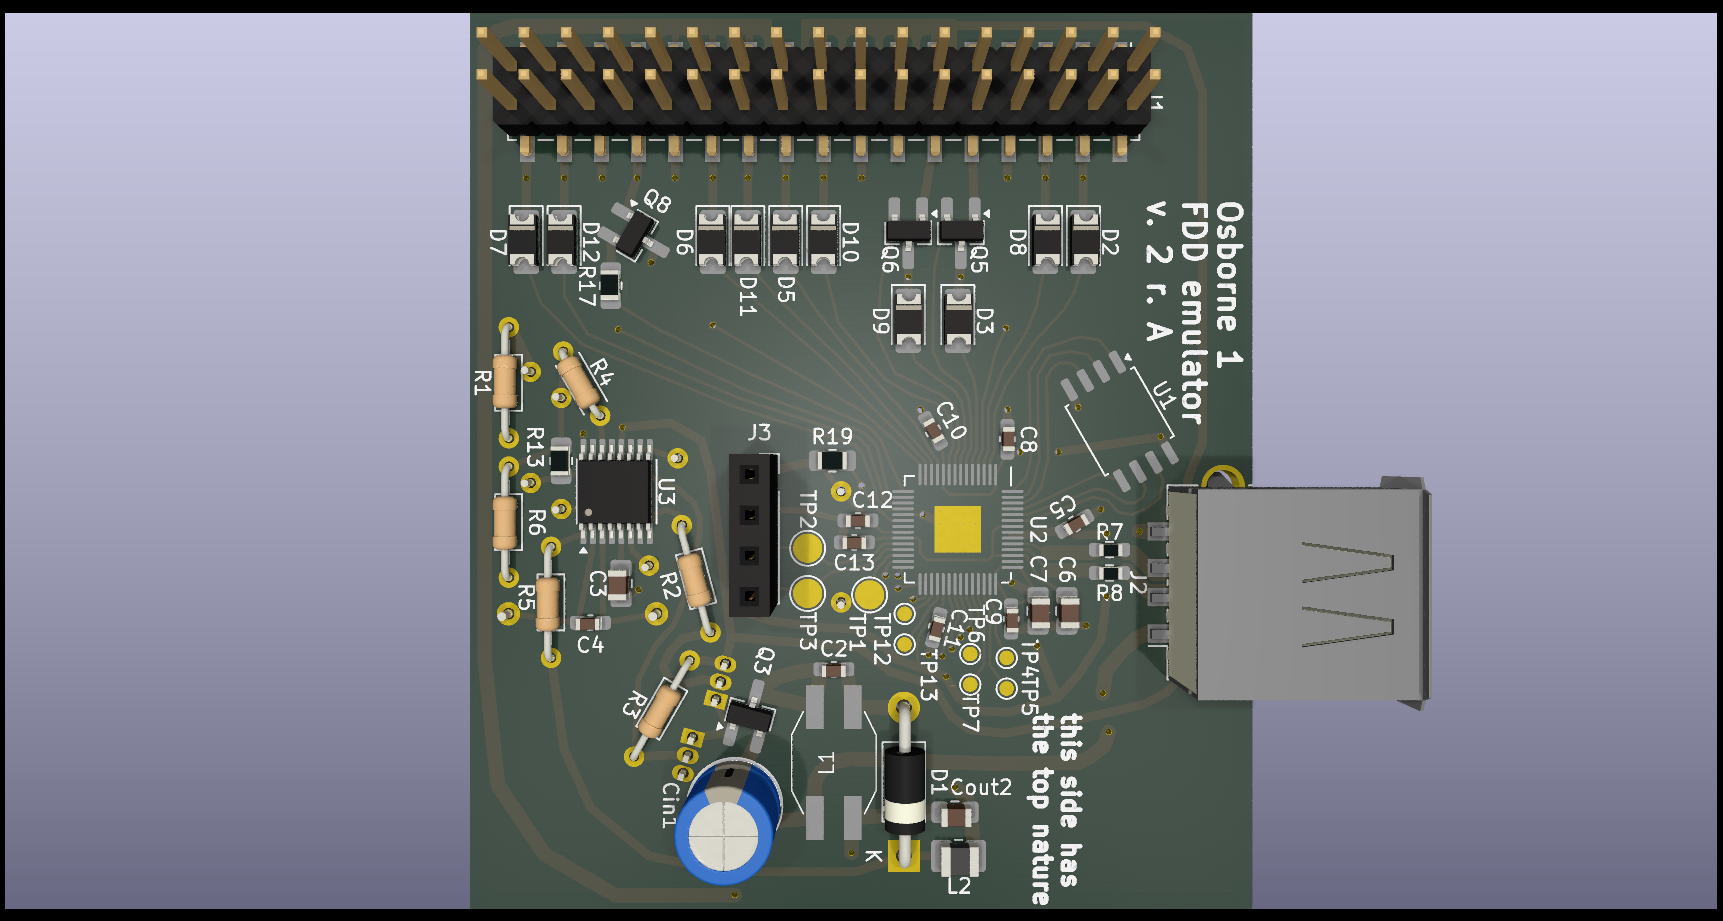
\includegraphics[height=5cm]{pcb-v2}
  \caption{Render of second version of PCB}
\end{figure}

Once we managed to get the RP2040 to run using the clock provided by
the Osborne 1, the increased power draw caused the tiny common-mode
choke in our power supply to saturate, causing excessive power draw
and insufficient voltage. To fix this we replaced it with a hand-wound
inductor we made earlier.

\begin{figure}
  \centering
  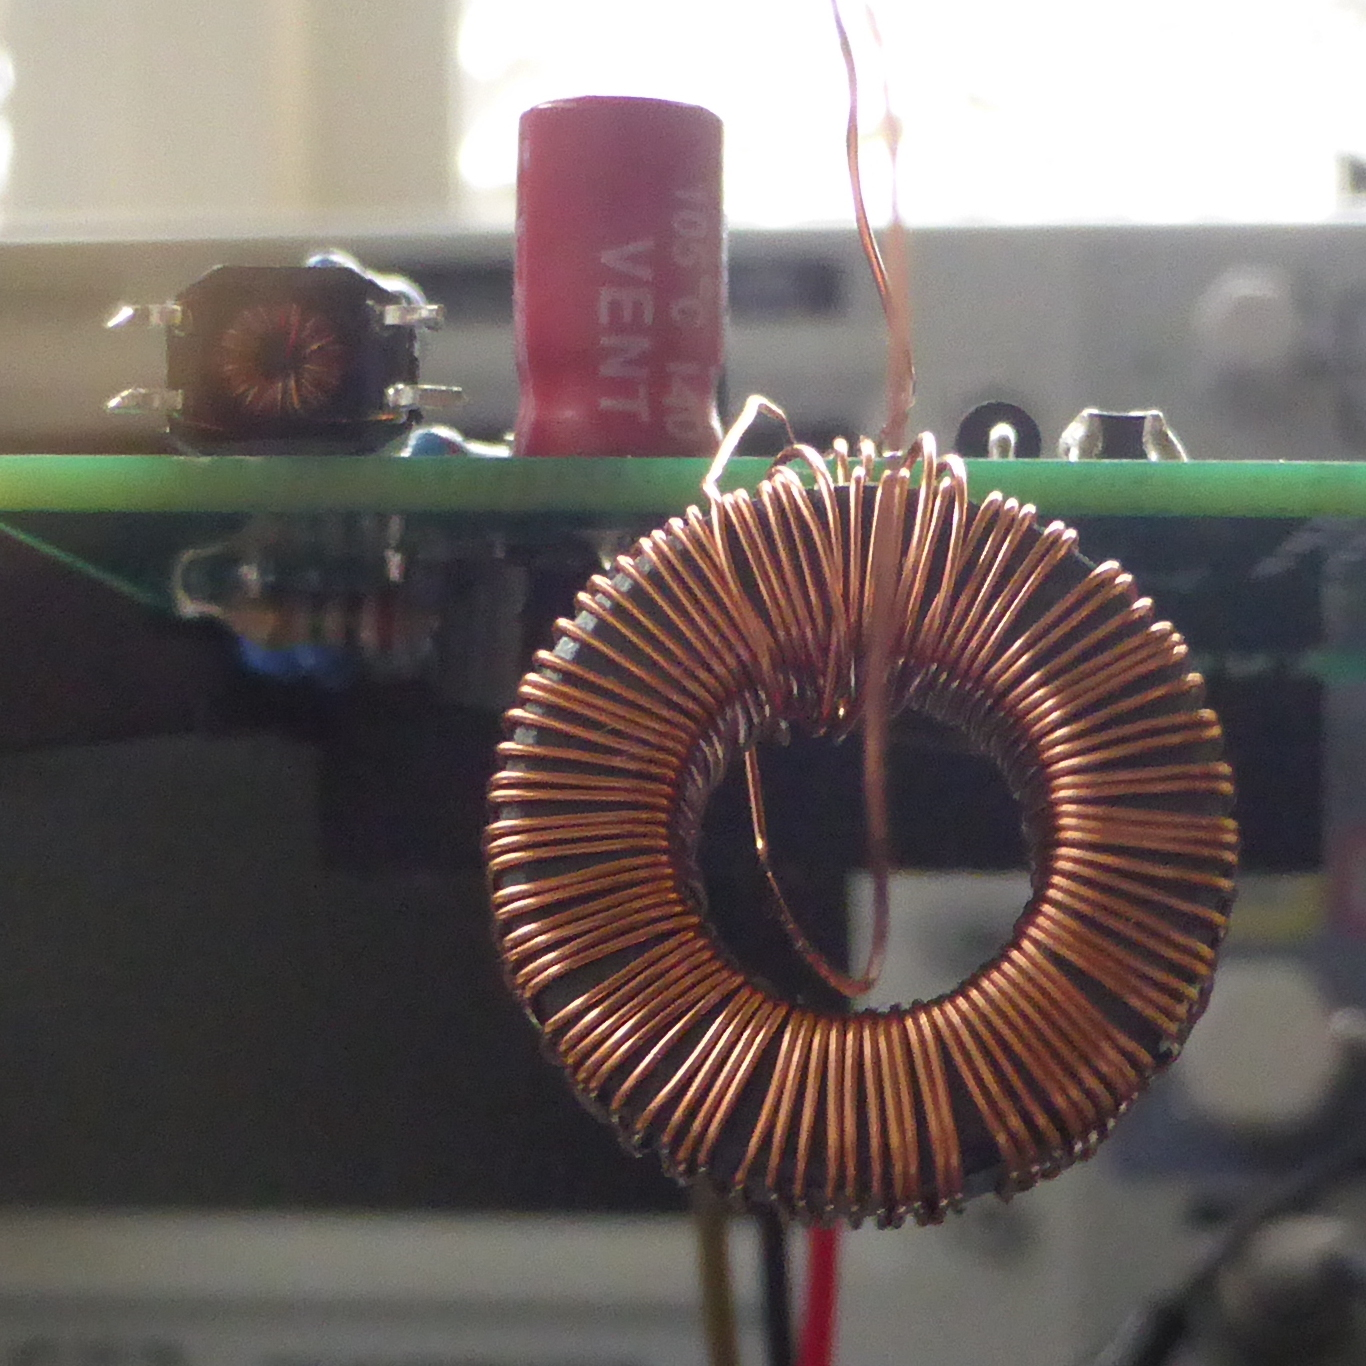
\includegraphics[height=5cm]{inductors}
  \caption[Inductors]{SMD common-mode choke (left) and hand-wound
    coupled inductors (right)}
\end{figure}

\begin{figure}
  \centering
  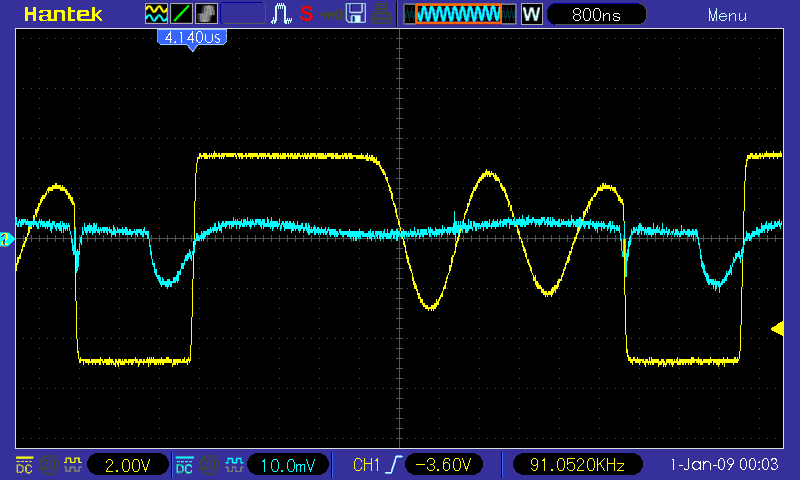
\includegraphics[height=3.5cm]{pic_25_1}\hfill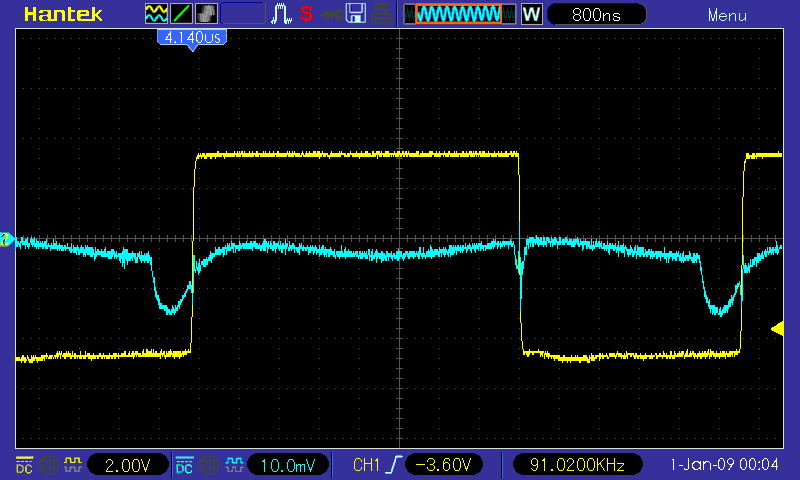
\includegraphics[height=3.5cm]{pic_25_4}
  \caption[Voltage and current traces with handwound inductors]{Diode
    anode voltage vs. time (yellow) and voltage across \qty{0.1}{\ohm}
    shunt (blue) with hand-wound inductors---On left under light load (in
    DCM) and on right under high load (in CCM)}
\end{figure}

\section {Design and Features}

For our project we decided to design our own PCBs and get them printed
by a commercial manufacturer. Our boards use a SEPIC (Single-Ended
Primary-Inductor Converter) SMPS to create a \qty{3.3}{\V} supply for
the RP2040 microcontroller, which has 2 cores and many other notable
features, such as a USB controller and PHY, and programmable I/O state
machines.

We wanted to be able to easily change what disks the emulator
emulated, so we decided to use a USB mass storage device to store
them. We haven't written the code to read and write disk images on a
USB device yet, but we plan to use the TinyUSB stack which is
integrated with the Pico SDK we are using.

So far we have been able to get the RP2040 to output a test signal
with mostly consistant timing, that mimics a floppy disk containing
deleted data, but we have not yet verified that the data is correct
and that any timing errors do not build up as the program runs.

\section{Challenges}

One of the challenges in using the RP2040 is that it doesn't have
enough RAM to fit an entire floppy disk in it when formatting is
included, so we needed to create a way to store the data that could
reduce the amount of redundant information, such as that contained in
the gaps (which are just one byte repeated many times), and allow
data to be loaded as it is needed and unloaded when it is unneeded. In
order to address the problem of memory allocation and the repeated
bytes, we use a system of linked lists containing elements of 3
different sizes---8, 24, and 72 bytes.

Another challenge was that the floppy disk drives send out the data
combined with the clock signal, as they are stored that way on the
floppy disk, which means that we either needed to store the clock
signal in the disk image (which wouldn't work well due to the
afformentioned memory constraint), or to be able to generate the clock
signal on the fly. Generating a clock signal is not particularly
difficult, but the problem is that the address marks, which are
important for the formatting of the drive, have missing clock bits,
meaning that we have to somehow send a byte with a missing clock
bit. Because our design used the PIO state machines to generate the
clock bits, this gave a challenge: to be able to switch from sending
data with the state machine's generated clock pulses to sending data
verbatim (at twice the speed), so that clock bits could be
deliberately omitted.

\end{document}
